\section{Overview}
Building on the dataset introduced in Chapter~\ref{ch:intro}, this chapter details the methodology employed to investigate climate change perceptions through social media data. The study uses a multimodal dataset of tweets, their replies, and associated images, focusing on two critical phases: \textbf{zero-shot experimentation} and \textbf{fine-tuning with soft labels}. The methodology is structured as follows:

\begin{enumerate}
    \item \textbf{Data Description and Preprocessing}: We further discuss how the dataset originally introduced in Chapter~\ref{ch:intro} has been filtered, cleaned, and prepared for analysis. This includes language detection, criteria for tweet selection, and other preprocessing steps to ensure high-quality input for downstream tasks.
    \item \textbf{Metrics}: We define evaluation metrics tailored to both zero-shot and fine-tuning paradigms.
    \item \textbf{Zero-Shot Experimentation}: We benchmark pre-trained language and vision models to select the best-performing architecture for zero-shot inference.
    \item \textbf{Weakly Supervised Learning}: We analyse weakly supervised approaches for emotion classification.
    \item \textbf{Fine-Tuning with Soft Labels}: The selected models are fine-tuned using soft labels generated using the best zero-shot text model.
    \item \textbf{Experimental Setup}: A comprehensive evaluation of model performance across experimental setups is conducted, with ablation studies to validate design choices.
\end{enumerate}

This structured approach ensures reproducibility while addressing challenges inherent to social media data, such as linguistic diversity, noise, and the subjective nature of climate change discourse.

\section{Data Description and Preprocessing}

\subsection{Dataset Source}
As noted in Chapter~\ref{ch:intro}, the dataset is derived from the study \emph{Towards Understanding Climate Change Perceptions: A Social Media Dataset} \cite{prasse2023towards}, comprising tweets, replies, and images posted on Twitter (X) in 2019. To capture temporal variations in climate change discourse, this work focuses on the months of \textbf{February and August 2019}.

\subsection{Data Filtering}
\begin{enumerate}
    \item \textbf{Temporal Filtering}: Tweets outside the months of February and August 2019 were excluded.
    \item \textbf{Language Filtering}:
    \begin{itemize}
        \item \textbf{Primary Tweets}: The \texttt{papluca/xlm-roberta-base-language-detection} model which is a fine-tuned variant of the XLM-RoBERTa \cite{DBLP:journals/corr/abs-1911-02116} classified tweet languages. Only English tweets were retained.
        \item \textbf{Replies}: Replies were pre-translated in the dataset to English in the original dataset, ensuring linguistic consistency.
    \end{itemize}
\end{enumerate}

\subsection{Preprocessing Pipeline}
\begin{enumerate}
    \item \textbf{Text Cleaning}:
    \begin{itemize}
        \item Removed URLs, hashtags, and user mentions using regex patterns.
        \item Retained emojis and punctuation to preserve sentiment cues.
    \end{itemize}
    \item \textbf{Multimodal Alignment}:
    \begin{itemize}
        \item Paired tweets with their corresponding replies and images using tweet IDs.
        \item Removed orphaned entries (e.g., tweets without replies or images).
    \end{itemize}
\end{enumerate}

\subsection{Final Dataset Statistics}
\begin{table}[h!]
\centering
\begin{tabular}{lcc}
\toprule
Metric                & February 2019 & August 2019 \\
\midrule
Total Tweets          & 1774          & 7,769      \\
English Tweets        & 1,673         & 7,345      \\
Replies               & 12,616        & 51,147     \\
Valid Images          & 1,673         & 7,345      \\
\bottomrule
\end{tabular}
\caption{Dataset Statistics for February and August 2019.}
\end{table}


This preprocessing ensures a focused, high-quality corpus for analyzing climate change perceptions while addressing linguistic and temporal complexities.

\section{Evaluation Metrics}

This research uses two sets of metrics: those that gauge ranking performance in zero-shot scenarios and those that measure distributional accuracy when models are fine-tuned with soft labels. 

\subsection{Zero-Shot Evaluation Metrics}
\label{subsec:zero-shot-metrics}

In the zero-shot setting, the model predicts labels without task-specific training. The following metrics emphasize ranking quality and semantic relevance:

\paragraph{Exact Match (EM) Accuracy}  
Measures the percentage of predictions for which the top-ranked label matches the ground truth. This provides a strict indicator of precision, especially for unambiguous classes.

\paragraph{Top-3 Accuracy}  
Calculates the fraction of instances where the correct label appears among the top three predictions. This reflects real-world recommendation scenarios where multiple plausible labels can be acceptable.

\paragraph{Ranked Score (RS)}  
Assigns a weighted score to each prediction, granting higher credit to correct labels placed earlier in the ranking. A correct prediction at rank $r$ earns \( \frac{1}{\log_2(r+1)} \), rewarding models that correctly prioritize relevant classes.

\paragraph{Normalized Discounted Cumulative Gain (NDCG@3)}  
Compares the predicted ranking with the ideal ranking, truncated to the top three positions. This standard information retrieval metric highlights the importance of correctly ordering the most relevant labels.
\begin{equation}
\text{NDCG@3} = \frac{\sum_{i=1}^{3} \frac{\text{rel}_i}{\log_2(i+1)}}{\sum_{i=1}^{3} \frac{\text{rel}_i^{\text{ideal}}}{\log_2(i+1)}}
\end{equation}

where $\text{rel}_i$ represents the relevance score of the item at rank $i$, and $\text{rel}_i^{\text{ideal}}$ denotes the relevance score in the ideal ranking (i.e., sorted in decreasing order of relevance).

\subsection{Fine-Tuning Evaluation Metrics}

For the fine-tuning phase, we obtain soft labels (probabilistic annotations) from weak supervision. Accordingly, these metrics assess how well predicted distributions align with the target distributions:

\paragraph{Cosine Similarity}  
Measures the cosine of the angle between predicted and target probability vectors. This captures directional alignment and is particularly useful for high-dimensional or multi-label tasks. It is computed as:
\begin{equation}
    \text{Cosine Similarity} = \frac{\sum_{i} P(i) Q(i)}{\sqrt{\sum_{i} P(i)^2} \sqrt{\sum_{i} Q(i)^2}}
\end{equation}

\paragraph{Kullback--Leibler Divergence (KLDiv)}  
Quantifies how one probability distribution $Q$ diverges from a true distribution $P$:
\begin{equation}
    D_{\mathrm{KL}}(P \parallel Q) = \sum_{i} P(i) \log \frac{P(i)}{Q(i)}
\end{equation}
It penalizes overconfident misclassifications, which is critical when working with noisy social media labels.

\paragraph{Mean Squared Error (MSE)}  
Computes the average squared difference between predicted probabilities $Q(i)$ and target probabilities $P(i)$:
\begin{equation}
    \mathrm{MSE} = \frac{1}{N} \sum_{i=1}^{N} \bigl(P(i) - Q(i)\bigr)^2
\end{equation}
MSE is sensitive to large deviations and helps maintain proper probability calibration, reducing the risk of assigning very high probabilities to rare classes.

\paragraph{Ranking-score}
Finally, to identify the best-performing experiments, we aggregated the mean values of metrics described above per experiment across both datasets and seeds. To standardize the evaluation, we normalized the metrics by preserving Cosine Similarity and inverting MSE and KL Divergence, ensuring higher values indicate better performance. A final ranking score was computed as the sum of these normalized metrics, and experiments were ranked accordingly. This approach provides a robust comparison, enabling the selection of the most effective configurations for further analysis.
\begin{equation}
\text{Ranking-score} = \text{Cosine Similarity} + (1 - \text{MSE}) + (1 - \text{KLDiv})
\end{equation}


\section{Zero-Shot Experimentation}

This section outlines our approach to selecting and evaluating zero-shot models for emotion classification in climate-change discourse. Our goal was to identify a pre-trained language model capable of handling informal, often noisy social media text when classifying emotions.

\subsection{Model Selection and Rationale}

We benchmarked five pre-trained models chosen for either their focus on social media content or their established zero-shot capabilities:

\begin{enumerate}
    \item \texttt{cardiffnlp/twitter-roberta-base-emotion-latest} \cite{antypas2023supertweetevalchallengingunifiedheterogeneous}
    \begin{itemize}
        \item Built on a \textbf{RoBERTa-base} architecture, fine-tuned for emotion detection on Twitter.
        \item Part of the \textbf{SuperTweetEval} benchmark, addressing multilabel scenarios (tweets can have multiple emotions).
        \item Trained on 154M tweets (up to December 2022) and fine-tuned on the \textbf{TweetEmotion} dataset.
    \end{itemize}
    
    \item \texttt{cardiffnlp/twitter-roberta-large-emotion-latest} \cite{antypas2023supertweetevalchallengingunifiedheterogeneous}
    \begin{itemize}
        \item A \textbf{RoBERTa-large} variant of the above model, offering greater capacity for contextual reasoning.
    \end{itemize}
    
    \item \texttt{facebook/bart-large-mnli} \cite{lewis2019bartdenoisingsequencetosequencepretraining}
    \begin{itemize}
        \item A BART model trained for Natural Language Inference (NLI), employed here for zero-shot classification.
        \item Uses an entailment-based approach \cite{DBLP:journals/corr/abs-1909-00161}, framing candidate labels (e.g., \textit{joy}) as hypotheses (e.g., “This text expresses joy”) and inferring probabilities from entailment scores.
    \end{itemize}
    
    \item \texttt{MoritzLaurer/mDeBERTa-v3-base-xnli-multilingual-nli-2mil7} \cite{laurer_less_2022}
    \begin{itemize}
        \item A multilingual DeBERTa model trained on cross-lingual NLI tasks, enabling zero-shot usage across different languages.
    \end{itemize}
    
    \item \texttt{MoritzLaurer/deberta-v3-large-zeroshot-v2.0} \cite{laurer_building_2023}
    \begin{itemize}
        \item A high-performing DeBERTa model fine-tuned to provide robust zero-shot classification.
    \end{itemize}
\end{enumerate}

\noindent \textbf{Why These Models?}
\begin{itemize}
    \item The CardiffNLP models were pre-trained for \textbf{social media emotion detection} on Twitter which makes then highly suitable for our task.
    \item BART and DeBERTa-based models provide \textbf{general-purpose zero-shot capabilities}, making them strong baselines for cross-domain generalization.
\end{itemize}

\subsection{Experimental Setup}

\subsubsection{Evaluation Dataset}
We sampled \textbf{99 English replies} from our corpus, manually assigning a single ground-truth emotion label to each. The labels followed Ekman’s six basic emotions—\textit{anger}, \textit{disgust}, \textit{fear}, \textit{joy}, \textit{sadness}, and \textit{surprise}—and their distribution is shown in Table~\ref{tab:manual_label_distribution}.

\begin{table}[ht]
    \centering
    \begin{tabular}{|c|c|}
        \hline
        \textbf{Manual Label} & \textbf{Count} \\
        \hline
        Anger     & 33 \\
        Joy       & 16 \\
        Disgust   & 15 \\
        Fear      & 13 \\
        Sadness   & 12 \\
        Surprise  & 10 \\
        \hline
    \end{tabular}
    \caption{Distribution of Manual Emotion Labels}
    \label{tab:manual_label_distribution}
\end{table}

\subsubsection{Procedure}
We evaluated each zero-shot model in two ways:

\paragraph{1) Primary Evaluation (Standard Metrics).}
All 99 samples were fed to each model, which returned a single emotion label per sample. We then computed the metrics described in Section~\ref{subsec:zero-shot-metrics}.

\paragraph{2) Secondary Evaluation (Confidence Filtering).}
We additionally filtered out low-confidence predictions by retaining only those with a confidence score above 0.9. This second analysis measured (a) the proportion of samples meeting the threshold and (b) the accuracy of high-confidence predictions.


\section{Weakly Supervised Learning}
\subsection{Zero-shot-classification-boost-with-self-training}
As outlined in Section \ref{sec:weakly_supervised_back}, \cite{gera_zero-shot_2022} proposed a self-training framework to enhance zero-shot text classification by iteratively fine-tuning models on their own high-confidence predictions. Their approach addresses the scarcity of labelled data by leveraging unlabeled corpora and class names alone, aligning with our goal of "classifying tweets into distinct emotion categories without task-specific labels". 

\subsubsection*{Reproduction of Gera et al.’s Methodology}
To validate the reproducibility of the original study, we reimplemented their workflow as follows:

\subsubsection*{Model and Dataset Selection}
\begin{itemize}
    \item We used the same off-the-shelf NLI models (RoBERTa-large, DeBERTa-v3) and datasets \textit{(AG’s news \cite{DBLP:journals/corr/ZhangZL15} and ISEAR \cite{Shao2015UniversalityVC})} as described in the original work.
    \item Weak supervision signals were derived solely from class names and unlabeled text, mirroring the zero-shot setup.
\end{itemize}

\subsubsection*{Self-Training Protocol}
\begin{itemize}
    \item \textbf{Pseudo-Label Generation:} For each dataset, we generated pseudo-labels by selecting the model’s most confident predictions (threshold: $\tau = 0.9$, as in the original study).
    \item \textbf{Token Masking:} We implemented the token masking heuristic to mask tokens with high semantic similarity to class names (using cosine similarity over SBERT embeddings).
    \item \textbf{Fine-Tuning:} Models were iteratively fine-tuned on pseudo-labeled batches (batch size: 8) for $K = 2$ iterations, retaining the original learning rate ($2 \times 10^{-5}$) and optimizer (AdamW).
\end{itemize}

\noindent
We adapted the framework to our task of \textit{classifying tweets into distinct emotion categories}.

\subsubsection*{Adaptations to the Self-Training Pipeline}
\begin{itemize}
    \item \textbf{Class Name Prompt Engineering:} To improve pseudo-label quality, we reformulated class names into natural language hypotheses (e.g., "The emotion in this text is joy" instead of "joy").
    \item \textbf{Cross-Task Sampling:} Since our task lacks related labelled datasets, we limited self-training to in-domain pseudo-labels, avoiding the cross-task degradation noted in \cite{gera_zero-shot_2022}.
\end{itemize}


\subsection{Loss Reweighting}  
\label{sec:loss_reweighting}  

To mitigate label noise from weak supervision, we implemented a confidence-based loss reweighting strategy described in sub-section \ref{subsubsec:loss_adjust}. This approach adjusts the influence of each training example based on confidence scores derived from the initial label generation process.  

\subsubsection{Implementation}  

This method consists of three key components:  

\begin{itemize}
    \item \textbf{Confidence-Weighted Loss Function}: The standard cross-entropy loss was modified to incorporate confidence scores as multiplicative weights. This ensured that higher-confidence samples contributed more to the learning process, while lower-confidence samples had a reduced impact.  

    \item \textbf{Data Integration Pipeline}: The training dataset combined weak labels, raw text, and confidence scores, represented as:  

    \begin{equation}
        \mathcal{D} = \{(\mathbf{x}_i, \tilde{y}_i, c_i)\}_{i=1}^N
    \end{equation}

    where $\tilde{y}_i$ denotes weak labels, and $c_i \in [0,1]$ represents the assigned confidence score.  

    \item \textbf{Adaptive Training Protocol}: We fine-tuned BERT-base using a structured approach:  
    \begin{itemize}
        \item Applied class-balanced sampling when enabled  
        \item Used the AdamW optimizer with a learning rate of $2\times10^{-5}$  
        \item Implemented early stopping based on validation performance  
    \end{itemize}
\end{itemize}  

\subsubsection{Theoretical Basis}  

This method aligns with a noise-robust learning objective:  

\begin{equation}
    \min_\theta \sum_{i=1}^N c_i \cdot \ell(f_\theta(\mathbf{x}_i), \tilde{y}_i)
\end{equation}

where $\ell$ is the cross-entropy loss, and $c_i$ acts as a weighting factor. This formulation prioritizes high-confidence samples while minimizing the influence of potentially incorrect labels.  

This strategy aimed to improve learning stability by focusing on reliable samples and reducing the effect of label noise in weakly supervised training.


\section{Fine-Tuning with Soft Labels}
\label{sec:finetuning}

This section presents our methodology for fine-tuning unimodal (text-only, image-only) and multimodal (text \& image) models using soft labels. The \textbf{CardiffNLP RoBERTa-Large} model exhibited the best performance in generating reliable emotion probability distributions under zero-shot conditions. We leveraged this optimal model to produce inference distributions across all replies linked to each parent tweet. For each original tweet, we then aggregated these reply-level probability distributions into a single soft-label signal by summation and normalization.
\newline

The resultant aggregated distributions serve as target supervisory signals for fine-tuning, where model parameters are updated by minimizing the Kullback–Leibler (KL) divergence between model outputs and these soft label distributions. This approach facilitates knowledge transfer from the robust zero-shot model while preserving the nuanced emotional gradients captured in the crowd-sourced replies. Figure~\ref{fig:architecture} illustrates the overall framework, including encoder components for each modality and the projection heads that map representations to the soft-label space. Training details regarding objective functions and implementation can be found in Section~\ref{sec:Experimental Setup}.

\subsection{Label Mapping to Ekman’s Six Emotions}
Since the CardiffNLP model originally yielded predictions for 11 emotion categories (e.g., \emph{love}, \emph{trust}, \emph{optimism}, \emph{anticipation}), we consolidated these into Ekman’s six basic emotions (\emph{anger, disgust, fear, joy, sadness, surprise}) to maintain consistency and interpretability. Table~\ref{tab:emotion_mapping} summarizes the mapping scheme, whereby categories such as \emph{love}, \emph{trust}, and \emph{optimism} are merged into \emph{joy}, and \emph{anticipation} is subsumed under \emph{surprise}. After merging, confidence scores for combined classes are normalized so that each distribution sums to 1.

\begin{table}[ht]
    \centering
    \begin{tabular}{|c|l|}
        \hline
        \textbf{Primary Emotion (Ekman)} & \textbf{Mapped Emotions (Original-11)} \\
        \hline
        Anger     & Anger \\
        Disgust   & Disgust \\
        Fear      & Fear \\
        Joy       & Joy, Love, Optimism, Trust \\
        Sadness   & Sadness \\
        Surprise  & Anticipation, Surprise \\
        \hline
    \end{tabular}
    \caption{Mapping of Emotions into Ekman Categories}
    \label{tab:emotion_mapping}
\end{table}

\paragraph{Rationale:}
\begin{enumerate}
    \item \textbf{Theoretical Robustness:} Ekman’s framework is widely recognized and reduces ambiguity in noisy, multicultural social media contexts.
    \item \textbf{Practical Efficiency:} Merging labels helps mitigate class imbalance (e.g., combining \emph{love}, \emph{optimism}, and \emph{trust} under \emph{joy}) and simplifies downstream training.
    \item \textbf{Domain Relevance:} In climate discourse, broad labels like \emph{anger} (e.g., policy opposition) or \emph{surprise} (e.g., reactions to disasters) provide actionable insights more readily than finer-grained categories.
    \item \textbf{Methodological Consistency:} Using a single taxonomy across different models enables uniform evaluation and aligns with prior work that employs Ekman’s classification.
\end{enumerate}

By consolidating all predictions under these six universal emotion categories, we ensure that both unimodal and multimodal models are trained on a well-defined and consistent label space.


\subsection{Architectural Overview}
In both cases i.e. Unimodal (Text or Image) and Multimodal, we attach a standard MLP as described below to the encoder output(s) for classification, unless specified otherwise. 

\subsubsection*{Projection Head (MLP)}
\begin{itemize}
    \item \textbf{Depth:} 2 layers.
    \item \textbf{Hidden Dimension:} 512.
    \item \textbf{Activation:} ReLU.
    \item \textbf{Output Layer:} Produces $6$ class probabilities (soft labels).
\end{itemize}


\begin{figure}[ht]
    \centering
    \begin{minipage}{0.49\textwidth}
        \centering
        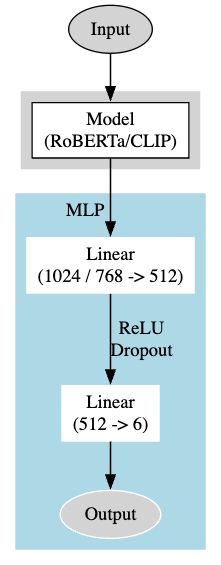
\includegraphics[height=0.5\textheight]{images/unimodal.png}
        \caption{Single Modality Architecture}
        \label{fig:arch1}
    \end{minipage}
    \hfill
    \begin{minipage}{0.49\textwidth}
        \centering
        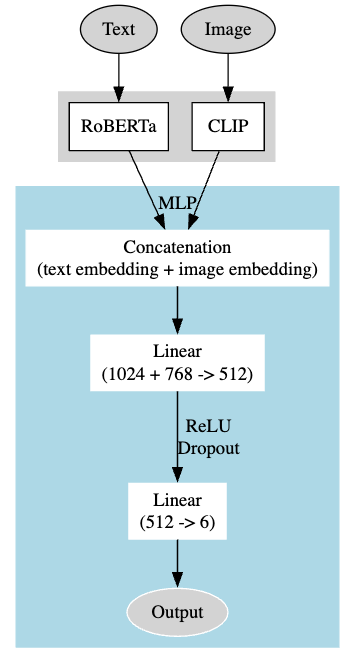
\includegraphics[height=0.5\textheight]{images/multimodal.png}
        \caption{Multimodal Fusion Architecture}
        \label{fig:arch2}
    \end{minipage}
    \caption{Finetuning setup with Base MLP}
    \label{fig:architecture}
\end{figure}

\subsubsection*{Unimodal-Text (Figure~\ref{fig:arch1})}
Uses a \textbf{Cardiffnlp RoBERTa-Large} encoder to produce text embeddings (1024-dim), followed by the standard projection head.

\subsubsection*{Unimodal Image (Figure~\ref{fig:arch1})}
Uses a \textbf{CLIP ViT-L/14} encoder to extract image embeddings (768-dim), again followed by the standard projection head.

\subsubsection*{Multimodal Fusion (Figure~\ref{fig:arch2})}
Combines text and image encoders from both unimodal settings in parallel. Text embeddings and image embeddings are concatenated. This fused representation (1792-dim) is passed to the standard projection head. For multimodal experiments, we tested many fine-tuned variations. The details are:

\begin{figure}[ht]
    \centering
    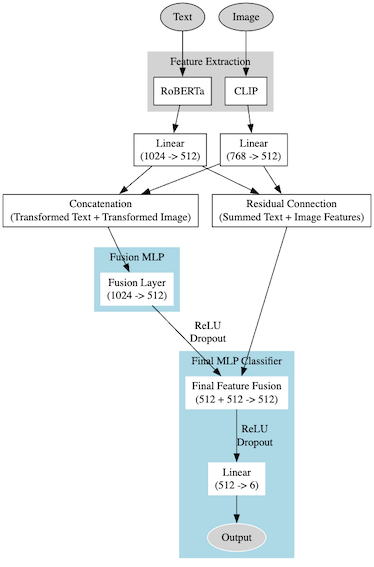
\includegraphics[height=0.6\textheight]{images/residual.png}
    \caption{Multimodal Residual fusion architecture}
    \label{fig:residual}
\end{figure}

\begin{itemize}
\item  \textbf{Encoder Tuning}
\begin{itemize}
    \item \textbf{Frozen text encoder:} Only freeze text encoder weights, fine-tune MLP and image encoder
    \item \textbf{Frozen image encoder:} Only freeze image encoder weights, fine-tune MLP and text encoder
    \item \textbf{Both encoders Frozen:} Freeze both encoder weights, only fine-tune MLP.
    \item \textbf{Full fine-tune:} Fine-tune MLP and both encoders.
    \item \textbf{Staggered-unfreezing} Unfreeze Image encoder weights after 2 epochs and unfreeze text encoder weights after 4 epochs.
\end{itemize}

\item \textbf{MLP variations}
\begin{itemize}
    \item Standard Projection Head (Figure~\ref{fig:arch2})
    \item Deeper (3-layer) MLP with ReLU Activation (hidden sizes 1024 and 512)
    \item Deeper (3-layer) MLP with GELU Activation (hidden sizes 1024 and 512)
\end{itemize}



\item \textbf{Fusion strategies}
\begin{itemize}
    \item Late Fusion - Concatenation of final layer embeddings of text and image models (Figure~\ref{fig:arch2})
    \item Residual Fusion (Concatenation + Residual Addition) (Figure~\ref{fig:residual})
\end{itemize}
\end{itemize}


All experiments were conducted on data from two distinct time intervals (February and August) for temporal robustness. These choices were combined systematically resulting in 320 unique experiment configurations (1280 in total for 2 datasets and 2 seeds)
\newline


A summary of the main architectural variations is given in Table~\ref{tab:architectural_variations}.

\begin{table}[ht]
    \centering
    \resizebox{\textwidth}{!}{%
    \begin{tabular}{lccc}
        \toprule
        \textbf{Component} & \textbf{Text-Based} & \textbf{Image-Based} & \textbf{Multimodal} \\
        \midrule
        Model & RoBERTa-large & CLIP ViT-L/14 & RoBERTa (Large/Base) + CLIP ViT-L/14 \\
        Input & Max 512 tokens & 224 × 224 pixels & Text: 512 tokens, Image: 224 × 224 \\
        Embedding Dim & 1024 & 768 & 1792 \\
        MLP Depth & 2 layers & 2 layers & 2 or 3 layers \\
        Hidden Sizes & 512 & 512 & 1024, 512 (3-layer MLP) \\
        Activation & ReLU & ReLU & ReLU or GELU \\
        Tuning Mode & Frozen or Fine-tuned & Frozen or Fine-tuned & Frozen, Fine-tuned or Staggered, \\
        Fusion Strategy & N/A & N/A & Concatenation / Residual Fusion \\
        \bottomrule
    \end{tabular}%
    }
    \caption{Architectural Variations}
    \label{tab:architectural_variations}
\end{table}

Our approach contrasts with baseline models which in our study are pre-trained zero-shot models, which are evaluated without any fine-tuning. Specifically:

\begin{itemize}
    \item For the \textbf{text-based approach}, the Baseline model is \textbf{CardiffNLP RoBERTa-Large}, which is used in a zero-shot setting.
    \item For the \textbf{image-based approach}, the Baseline model is \textbf{CLIP ViT-L/14}, applied without fine-tuning.
    \item For the \textbf{multimodal approach}, the Baseline predictions are obtained by averaging the outputs from these two unimodal Baseline models.
\end{itemize}


\section{Experimental Setup}
\label{sec:Experimental Setup}
This section details the computing environment, hyperparameter selection, reproducibility measures, and monitoring tools used for the experiments.

\subsection*{Hardware and Software Configuration}
\begin{itemize}
    \item \textbf{Hardware:} Two NVIDIA RTX A6000 GPUs with 48~GB VRAM each.
    \item \textbf{Programming Language:} Python 3.9
    \item \textbf{Key Libraries:}
    \begin{itemize}
        \item PyTorch 2.5.0 with CUDA 11.8
        \item HuggingFace Transformers 4.44.2
        \item NumPy 1.26.4, pandas 2.2.2
        \item scikit-learn 1.5.1 for evaluation metrics
        \item TensorBoard 2.18.0 provided real-time loss and accuracy curves
    \end{itemize}
\end{itemize}

\subsection*{Training Configuration and Hyperparameters}
A systematic approach was employed to explore and validate hyperparameter choices:
\begin{itemize}
    \item \textbf{Objective Function:} KL divergence to match soft-label distributions.
    \item \textbf{Optimizers:} Compared Adam vs. AdamW (decoupled weight decay $\lambda=0.01$), with $\beta_1=0.9$, $\beta_2=0.999$.
    \item \textbf{Learning Rates:} \{ $1 \times 10^{-5}$, $5 \times 10^{-6}$ \}.
    \item \textbf{Batch Size:} Typically 16 per GPU.
    \item \textbf{Epochs:} 2, 5 and 10
    \item \textbf{Regularization:}
    \begin{itemize}
        \item Dropout \{0.3, 0.5\} within MLP layers.
        \item Weight decay (AdamW).
    \end{itemize}
\end{itemize}

\subsection*{Reproducibility Protocol}
\begin{itemize}
    \item All experiments were conducted using two distinct random seeds (42 and 7) to ensure reproducibility.
    \item Randomness was controlled by setting the same seed for Python's random module, NumPy, PyTorch, and CUDA operations.
    \item Identical initialization and data splits were maintained across all runs.
\end{itemize}





